\hypertarget{cap1}{}
\chapter{Título do capítulo 1}

Escrever brevemente sobre o que será abordado nesse capítulo.

\section{Título da seção}

As figuras \ref{s-01} e \ref{s-02} mostram a distribuição de um
conjunto de moléculas formando a fase nemática uniaxial. Apesar de
ambas possuírem a mesma direção orientacional, definida pelo diretor,
$\vec{n}$, existe uma visível diferença no grau de ordenamento entre
elas.
\begin{figure}[!htb]
	\centering
	\subfloat[]{\label{s-01}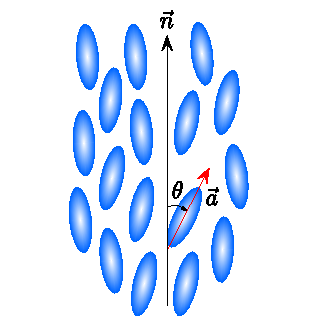
\includegraphics[scale= 1.0]{fig/s-01}}
	\hspace{1cm}
	\subfloat[]{\label{s-02}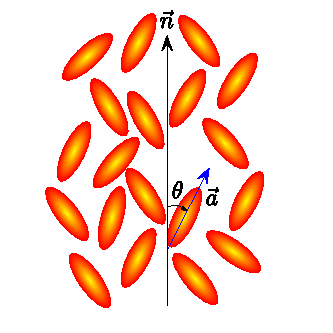
\includegraphics[scale= 1.0]{fig/s-02}}
	\caption{As figuras apresentam mesma direção orientacional,
contudo diferentes graus de ordenamento. Podemos observar que a figura
(a) possui uma menor dispersão da média, definida pelo diretor,
do que a figura (b).}
	\label{fig1}
\end{figure}

Este grau de alinhamento pode ser descrito por uma função
distribuição normalizada\footnote{$\oint f(\theta)\, d\Omega =
\int_{0}^{2\pi} \int_{0}^{\pi} f(\theta)\, {\rm sen}\, \theta\,
d\theta\, d\phi = 1$}, $f(\theta)\, d\theta$, que fornece a
probabilidade de encontrar o eixo principal de uma molécula, $\vec{a}$,
formando um ângulo entre $\theta$ e $\theta + d\theta$ com o diretor.
Devido à simetria cilíndrica das moléculas, a função distribuição
é independente do ângulo azimutal, $\phi$.

O parâmetro de ordem tensorial $Q_{ij}$ pode ser representado por uma
matriz, ou seja,
\begin{equation*} 
	Q_{ij}=\left(
		\begin{array}{ccc} 
			-(S + P)/2 & 0          & 0\\ 
			0          & -(S - P)/2 & 0\\ 
			0          & 0          & S
		\end{array}\right)\ ,
\end{equation*}
onde $S$ e $P$ são os parâmetros de ordem escalares. A equação
\eqref{eq2} mostra como fazer uma equação dentro de uma caixa
\begin{equation}
	\boxed{\Tilde{\mathcal{F}}_{\rm LdG}= \frac{\sigma}{2} \, {\rm
Tr}\Tilde{\bf Q}^2 - {\rm Tr}\Tilde{\bf Q}^3 + \frac{1}{2}\, ({\rm
Tr}\Tilde{\bf Q}^2)^2 + ... }\ .
	\label{eq2}
\end{equation}

Não esqueça de ver o \hyperlink{apen}{Apêndice A}.
